\chapter{Resultados}
\label{cap:resultados}

Este capítulo descreve primeiro o protocolo de execução e a linha de base, obtida com a configuração do trabalho de \citeonline{Souza2023}. Em seguida, os resultados da campanha experimental são organizados pelos quatro eixos de otimização: organização do código, paralelismo, automação de hiperparâmetros e segmentadores. O capítulo termina com a verificação dos requisitos e a discussão dos resultados.

\section{Protocolo de Execução}
\label{sec:resProtocolo}

Todos os experimentos foram executados no ambiente descrito na \autoref{sec:ambiente}, em modo determinístico. Salvo a comparação com o trabalho original (\autoref{qua:linhaBase}) e as acurácias citadas nas medições de paralelismo, obtidas com uma única semente (42), os resultados de acurácia são médias de execuções com sementes distintas (5 sementes nos retreinos finais e 3 nas comparações de estratégias de busca, na fração do treino e na análise do identificador) e, onde o desvio foi registrado, são apresentados com o desvio padrão populacional entre elas. Os tempos são médias de repetições da mesma configuração; nas medições de paralelismo em CPU, o PyTorch foi restrito a uma thread interna, salvo onde indicado, para que $N$ threads ou processos de trabalho correspondessem a $N$ núcleos, e os pools foram criados e aquecidos fora do intervalo medido, com o custo de partida registrado à parte.

Os experimentos de hiperparâmetros e de segmentadores treinam com 10\% do conjunto de treino (871 amostras em Indian Pines), com teto de 200 épocas, parada por estagnação de 10 épocas e meta de acurácia de validação de 0,95; a validação e o teste permanecem inteiros. Treinar com essa fração torna cada \textit{trial} 5,7 vezes mais barato (6,0 s contra 34,3 s por execução em Indian Pines; \autoref{qua:fracaoTreino}); o ganho da busca com o treino completo não foi medido. O custo dessa redução em acurácia, medido com a configuração herdada, está na \autoref{sec:resLinhaBase}. Os demais experimentos usam o treino completo.

\section{Linha de Base}
\label{sec:resLinhaBase}

Com a configuração do próprio notebook, a reimplementação obtém em University of Pavia OA 0,9763, AA 0,9579 e Kappa 0,9685, e repete esses valores, o histórico de perda por época e os pesos finais em execuções sucessivas. A execução registrada no notebook original, que não fixa a semente da inicialização e do treino da rede, obteve OA 0,9819, AA 0,9735 e Kappa 0,9760. Os dois frameworks não partem dos mesmos pesos, de modo que a igualdade numérica não é esperada, e uma diferença de 0,56 ponto na OA entre uma execução de cada lado não permite separar o efeito da implementação do efeito da inicialização. O que sustenta as comparações seguintes é que a reimplementação preserva a arquitetura (37.577 parâmetros nessa cena, os mesmos do modelo Keras), o PCA, a divisão dos dados, com as mesmas sementes e as mesmas 3.208 amostras de teste, e os hiperparâmetros de treino, e que cada configuração produz sempre o mesmo resultado; nas comparações seguintes, só a regra de parada antecipada difere da do original (\autoref{subsec:desTreino}).

O \autoref{qua:linhaBase} compara a configuração herdada, executada pela reimplementação com a política de parada da \autoref{subsec:desTreino} e o treino completo, com os valores reportados por \citeonline{Souza2023}. Os valores do trabalho original são superiores --- por menos de 1 ponto de OA em Indian Pines e Salinas Valley, 1,6 ponto em University of Pavia e 7,2 pontos de AA em Indian Pines, onde as classes raras pesam mais ---, o que é coerente com o modo como foram obtidos: o autor relata ter ajustado, por conjunto de dados, a paciência da parada antecipada e outros parâmetros de treino ao buscar o melhor resultado \cite{Souza2023}, enquanto aqui a mesma política vale para as três cenas. A comparação é entre uma execução de cada lado, com a semente 42 na reimplementação.

\begin{quadro}[H]
    \centering
    \caption{Configuração herdada: valores reportados no trabalho original e obtidos pela reimplementação}
    \begin{tabular}{|p{0.20\textwidth}|c|c|c|c|c|c|}
        \hline
        \rowcolor[HTML]{C0C0C0}
        & \multicolumn{3}{c|}{\textbf{Reportado}} & \multicolumn{3}{c|}{\textbf{Reimplementação}} \\
        \hline
        \rowcolor[HTML]{C0C0C0}
        \textbf{Cena} & \textbf{OA} & \textbf{AA} & \textbf{Kappa} & \textbf{OA} & \textbf{AA} & \textbf{Kappa} \\
        \hline
        Indian Pines & 0,9142 & 0,8956 & 0,9019 & 0,9051 & 0,8237 & 0,8914 \\
        \hline
        University of Pavia & 0,9928 & 0,9866 & 0,9905 & 0,9772 & 0,9644 & 0,9698 \\
        \hline
        Salinas Valley & 0,9965 & 0,9970 & 0,9962 & 0,9938 & 0,9956 & 0,9931 \\
        \hline
    \end{tabular}
    \captionsetup{justification=raggedright}
    \caption*{Fonte: Elaborado pelo autor, com os valores reportados por \citeonline{Souza2023}. Reimplementação: semente 42, treino completo}
    \label{qua:linhaBase}
\end{quadro}

O \autoref{qua:fracaoTreino} mostra o custo de treinar com menos amostras, medido em Indian Pines com a configuração herdada. Com 10\% do treino, a OA cai 14,3 pontos percentuais e a AA, 23,0, enquanto o tempo por execução cai de 34,3 s para 6,0 s. Os resultados com 10\% do treino, portanto, não são comparáveis em valor absoluto aos do \autoref{qua:linhaBase}; são comparáveis entre si, porque todas as condições comparadas em cada experimento usam a mesma fração.

\begin{quadro}[H]
    \centering
    \caption{Custo de treinar com uma fração do conjunto de treino (Indian Pines, 3 sementes, teto de 60 épocas)}
    \begin{tabular}{|c|c|c|c|c|c|}
        \hline
        \rowcolor[HTML]{C0C0C0}
        \textbf{Fração} & \textbf{Amostras} & \textbf{OA} & \textbf{AA} & \textbf{Kappa} & \textbf{Tempo (s)} \\
        \hline
        100\% & 8.711 & 0,9016 $\pm$ 0,0016 & 0,8308 & 0,8877 & 34,3 \\
        \hline
        50\% & 4.356 & 0,8643 $\pm$ 0,0140 & 0,7310 & 0,8448 & 18,8 \\
        \hline
        25\% & 2.179 & 0,8270 $\pm$ 0,0105 & 0,6755 & 0,8021 & 11,4 \\
        \hline
        10\% & 871 & 0,7586 $\pm$ 0,0109 & 0,6006 & 0,7227 & 6,0 \\
        \hline
        5\% & 435 & 0,6810 $\pm$ 0,0131 & 0,5322 & 0,6334 & 4,0 \\
        \hline
    \end{tabular}
    \captionsetup{justification=raggedright}
    \caption*{Fonte: Elaborado pelo autor}
    \label{qua:fracaoTreino}
\end{quadro}

\section{Organização do Código}
\label{sec:resOrganizacao}

O principal resultado deste eixo é qualitativo: a reimplementação fiel à arquitetura, ao PCA, à divisão dos dados e aos hiperparâmetros de treino do original, com a regra de parada antecipada trocada (\autoref{subsec:desTreino}), e a reprodutibilidade das execuções, em que a mesma configuração produz sempre o mesmo resultado. A organização, porém, também tornou visíveis três defeitos: dois que teriam contaminado resultados em silêncio e um que interrompia a campanha com um erro que não apontava a causa.

\textbf{Não determinismo do LSC.} A implementação paralela do LSC no OpenCV desempata pela ordem das threads, e duas chamadas com a mesma imagem e os mesmos parâmetros devolviam rótulos diferentes em 388 pixels de Indian Pines; SEEDS, SLIC e Watershed não tinham o problema. Com o LSC no espaço de busca, a pontuação de um mesmo \textit{trial} variava entre execuções, e as estratégias adaptativas amplificavam a variação até trocarem de vencedor: a mesma campanha de TPE chegou a 0,8713 de validação em uma execução e a 0,7711 em outra, na qual, com 200 épocas por \textit{trial}, ficou atrás da busca aleatória (0,8075) e do algoritmo genético (0,8309). O defeito foi isolado por eliminação --- treino com configuração fixa determinístico, amostradores determinísticos com pontuações fixas e, por fim, a comparação direta das saídas dos segmentadores --- e corrigido restringindo o OpenCV a uma thread, com custo nulo (38,6 ms por segmentação, contra 39,1 ms com 32 threads). As medições anteriores à correção que envolviam o LSC foram descartadas, exceto três, assinaladas: o LSC sob otimização conjunta (\autoref{qua:segmentadores}), o LSC com a CNN fixa em University of Pavia e as métricas estruturais do LSC no \autoref{qua:estruturaSeg}.

\textbf{Gerador aleatório compartilhado entre threads.} Quando as partições da cena treinam em threads de um mesmo processo, todas consomem o mesmo gerador aleatório global do PyTorch, na inicialização dos pesos e nas máscaras de \textit{dropout}, em ordem imprevisível. Execuções que deveriam ser idênticas variaram até 3,51 pontos de OA, enquanto as execuções sequenciais e em processos repetiram o valor exatamente. Não há semente que corrija isso sem dar um gerador a cada partição, que é o que processos fazem por construção; por isso, toda acurácia de partição reportada vem de execuções sequenciais ou em processos.

\textbf{Número mínimo de componentes.} A geração das opções de PCA do espaço de busca usava um piso herdado da composição RGB (3 componentes), e não o da rede, que exige 15. Em University of Pavia e Salinas Valley, cuja receita é de 15 componentes, a busca gerava a opção de 8, e o primeiro \textit{trial} que a sorteava interrompia a campanha com um erro do PyTorch que apontava para a convolução, e não para a causa. O piso passou a ser derivado dos próprios \textit{kernels} da rede.

Quanto à memória, cada \textit{trial} da busca retinha 2,5 MB em Indian Pines, 5,1 MB em University of Pavia e 6,5 MB em Salinas Valley. Com a liberação dos resultados que não são o melhor corrente, a memória do processo cresceu 16 MB ao longo de uma campanha de 180 \textit{trials} (de 1.894 MB para 1.910 MB). Na CNN 1D, cujo conjunto de dados é pequeno, reter todos os resultados seria incômodo, mas não impeditivo (cerca de 450 MB em 180 \textit{trials} de Indian Pines); a liberação serve para manter constante a memória da campanha.

\section{Paralelismo}
\label{sec:resParalelismo}

\subsection{Entre os Ramos do Pré-processamento}

O \autoref{qua:ramos} e a \autoref{fig:ramos} mostram o tempo de cada ramo e o ganho de executá-los concorrentemente. A segmentação domina o pré-processamento (de 78\% a 93\% do tempo serial) e, pelo teto da \autoref{sec:concorrencia}, o ganho máximo fica entre 1,08$\times$ e 1,29$\times$. Com threads, Salinas Valley atinge 1,22$\times$ contra um teto de 1,21$\times$, ou seja, a implementação está no limite do que o desenho permite; em Indian Pines, o ganho fica em 1,05$\times$, contra um teto de 1,29$\times$, e em University of Pavia, onde o teto é 1,08$\times$, a sobrecarga de coordenação já basta para anular o ganho (0,95$\times$). Com processos, o custo de criar o processo filho e serializar de 8,4 MB a 45,3 MB de dados faz o pré-processamento ficar de 1,3 a 4,5 vezes mais lento.

\begin{quadro}[H]
    \centering
    \caption{Paralelismo entre os ramos do pré-processamento (5 repetições, tempos em segundos)}
    \begin{tabular}{|l|c|c|c|c|c|c|}
        \hline
        \rowcolor[HTML]{C0C0C0}
        \textbf{Cena} & \textbf{Espectral} & \textbf{Espacial} & \textbf{Sequencial} & \textbf{Threads} & \textbf{Processos} & \textbf{Teto} \\
        \hline
        Indian Pines & 0,037 & 0,129 & 0,166 & 1,05$\times$ & 0,22$\times$ & 1,29$\times$ \\
        \hline
        University of Pavia & 0,072 & 0,899 & 0,971 & 0,95$\times$ & 0,75$\times$ & 1,08$\times$ \\
        \hline
        Salinas Valley & 0,142 & 0,680 & 0,822 & 1,22$\times$ & 0,74$\times$ & 1,21$\times$ \\
        \hline
    \end{tabular}
    \captionsetup{justification=raggedright}
    \caption*{Fonte: Elaborado pelo autor. Teto: tempo sequencial dividido pelo tempo do ramo espacial. Como o teto é calculado com tempos médios, uma medição pode ficar ligeiramente acima dele, como em Salinas Valley}
    \label{qua:ramos}
\end{quadro}

\begin{figure}[H]
    \centering
    \captionsetup{justification=centering}
    \caption{Tempo de cada ramo do pré-processamento e \textit{speedup} medido contra o teto teórico}
    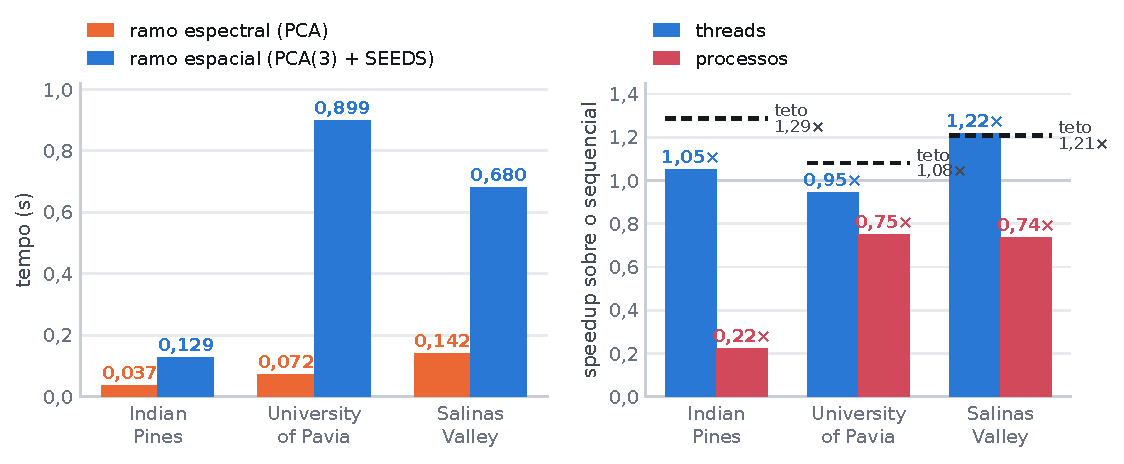
\includegraphics[width=\textwidth]{assets/resultados/ramos_preprocessamento.pdf}
    \captionsetup{justification=raggedright}
    \caption*{Fonte: Elaborada pelo autor}
    \label{fig:ramos}
\end{figure}

Há, porém, um limite mais forte que o teto dos ramos. Em Indian Pines, o pré-processamento inteiro leva 0,193~s, contra 20,13~s de treino, e representa 0,9\% do tempo de uma execução; pela lei de Amdahl, nenhuma otimização dele muda o tempo total em mais de 0,9\%. Esse resultado motivou a partição da cena, que paraleliza o treino, etapa que concentra o tempo de execução; a fusão concorrente, apresentada depois, atua sobre a segmentação e a inferência.

\subsection{Threads Internas do PyTorch}

Antes de paralelizar o treino entre partições, foi medido o paralelismo que o próprio PyTorch oferece dentro de cada operação. Em uma medição avulsa, fora dos experimentos do \autoref{qua:experimentos}, 25 épocas de treino em Indian Pines, em CPU, levaram 11,67 s com as 16 threads padrão, 7,81 s com 8, 7,90 s com 4, 8,45 s com 2 e 8,55 s com uma única thread. A rede é pequena demais para que dividir cada operação compense: com 16 threads, o treino fica 1,37 vez mais lento que com uma. O GIL impõe um limite de outra natureza, que pesa sobre o código Python executado em threads, e não sobre as threads internas do PyTorch, que executam código nativo: em outra medição avulsa, quatro threads executando um laço em Python puro levaram 0,91 s, contra 1,01 s em sequência, enquanto quatro multiplicações de matrizes em código nativo caíram de 0,80 s para 0,28 s.

\subsection{Por Partição da Cena}

O \autoref{qua:poolQuente} e a \autoref{fig:poolQuente} mostram o \textit{speedup} da partição da cena no modo independente, em que cada partição treina seu modelo, sempre contra a execução sequencial das mesmas partições no mesmo dispositivo, a CPU. Nessas medições, do experimento 13 (\autoref{qua:experimentos}), o treino usa lote 64 e teto de 25 épocas, com uma thread do PyTorch por partição.

\begin{quadro}[H]
    \centering
    \caption{\textit{Speedup} da partição da cena sobre a execução sequencial das mesmas partições (Indian Pines, 25 épocas)}
    \begin{tabular}{|p{0.32\textwidth}|c|c|c|c|}
        \hline
        \rowcolor[HTML]{C0C0C0}
        \textbf{Executor} & \textbf{N = 2} & \textbf{N = 4} & \textbf{N = 8} & \textbf{N = 16} \\
        \hline
        Threads & 1,61$\times$ & 0,61$\times$ & 0,23$\times$ & 0,23$\times$ \\
        \hline
        Processos, pool frio & 1,20$\times$ & 1,46$\times$ & 1,37$\times$ & 1,05$\times$ \\
        \hline
        Processos, pool quente & 1,86$\times$ & 2,87$\times$ & 3,68$\times$ & 4,47$\times$ \\
        \hline
    \end{tabular}
    \captionsetup{justification=raggedright}
    \caption*{Fonte: Elaborado pelo autor}
    \label{qua:poolQuente}
\end{quadro}

\begin{figure}[H]
    \centering
    \captionsetup{justification=centering}
    \caption{\textit{Speedup} da partição da cena por executor e número de partições}
    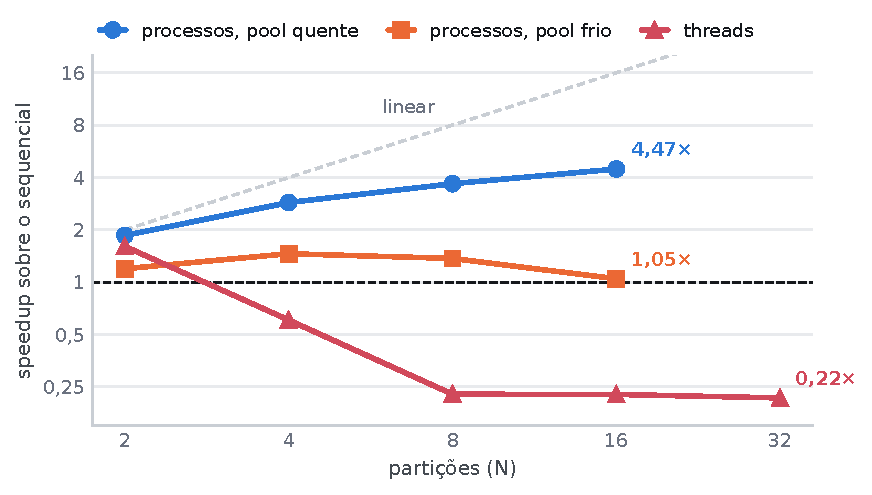
\includegraphics[width=0.85\textwidth]{assets/resultados/pool_quente.pdf}
    \captionsetup{justification=raggedright}
    \caption*{Fonte: Elaborada pelo autor}
    \label{fig:poolQuente}
\end{figure}

Três leituras se destacam. A primeira é que threads não escalam no treino: o laço de treino de uma rede pequena em CPU é dominado por código Python, que disputa o GIL, e a partir de 4 partições as threads ficam mais lentas que a execução sequencial. A segunda é que a forma de medir decide a conclusão: com o pool criado e destruído dentro da medição, como na primeira versão do experimento, cada medição inclui a inicialização de $N$ interpretadores, e o \textit{speedup} em $N = 16$ parece nulo (1,05$\times$); com o pool aquecido, o mesmo arranjo entrega 4,47$\times$. O custo de partida chega a 78\% do tempo do pool frio em $N = 16$ e foi registrado à parte, para que continue visível. A terceira é que o desenho escala, mas a máquina não acompanha: uma partição que leva 0,80 s sozinha leva 2,65 s com 16 executando juntas, 3,30 vezes mais lenta. A causa provável é a disputa de banda de memória e de \textit{cache} entre os processos, que não foi medida diretamente; outras causas, como a redução da frequência dos núcleos sob carga, não foram descartadas.

Em processos, a partição produz o mesmo resultado que a execução sequencial das mesmas partições: a OA é idêntica nas duas para $N = 2$, 4, 8 e 16. O paralelismo por processos, porém, esbarra em memória antes de esbarrar em núcleos. No experimento 13, cada processo criado por \textit{spawn} ocupa cerca de 481 MB de memória proporcional, e 32 processos exigiriam 15,4 GB em uma máquina de 15,8 GB; a configuração foi recusada antes de executar. Há também um limite de dados: com 32 partições restam cerca de 272 amostras de treino em cada uma, e a OA do modo independente cai para 0,850, contra 0,900 a 0,915 com 2 a 16 partições. Como cada partição treina e avalia um modelo próprio, com lote 64, 25 épocas e uma única semente, essas acurácias servem apenas para comparar números de partições entre si, e não são comparáveis à do modelo único. No modo replicado (experimento 11), em que um único modelo treinado com a cena inteira é usado para inferir as partições, a OA é idêntica à do modelo único (0,883), mas a inferência representa 0,4\% da execução, e não há o que ganhar.

\subsection{Fusão Concorrente}
\label{subsec:resFusao}

A fusão concorrente foi medida na inferência de todos os pixels rotulados de cada cena --- 10.249 em Indian Pines, 42.776 em University of Pavia e 54.129 em Salinas Valley ---, com o modelo da configuração herdada treinado com o treino completo. As referências são duas: o lote, que segmenta a cena e depois infere todos os pixels de uma vez, como faz o fluxo original, executado com uma e com 16 threads internas do PyTorch; e a execução sequencial por blocos, na mesma granularidade das tarefas concorrentes. O esquema foi medido nas duas formas da \autoref{subsec:fusaoConcorrente}, como no esquema e na variante desacoplada, com 1, 2, 4, 8 e 16 threads de trabalho, blocos de 1, 64 e 1.024 posições --- o bloco de uma posição apenas em Indian Pines, porque nas outras cenas seriam dezenas de milhares de tarefas por execução --- e as duas extensões da seção crítica, com 5 repetições por configuração (3 com bloco de uma posição). Em todas as 723 execuções, 660 delas da fusão concorrente, os identificadores lidos do mapa foram os mesmos usados no treino e as classes previstas foram idênticas às do lote.

O limite do esquema é dado pela segmentação: se toda a inferência fosse escondida atrás dela, o tempo de parede seria o próprio tempo do SEEDS, e o \textit{speedup} sobre o lote seria a razão entre o tempo do lote e o da segmentação. Esse teto, calculado com o tempo médio da segmentação nas execuções sequenciais por blocos, é de 2,98$\times$ em Indian Pines, onde a segmentação leva 0,111 s, mas de apenas 1,21$\times$ em University of Pavia e 1,49$\times$ em Salinas Valley, onde ela leva 0,869 s e 0,670 s e domina o tempo do lote. O \autoref{qua:fusao} e a \autoref{fig:fusaoSpeedup}, ambos com a seção crítica como no esquema, mostram o \textit{speedup} obtido sobre o lote com uma thread do PyTorch.

\begin{quadro}[!htbp]
    \centering
    \caption{\textit{Speedup} da fusão concorrente sobre o lote com uma thread do PyTorch, por número de threads de trabalho}
    \resizebox{\textwidth}{!}{%
    \begin{tabular}{|l|l|c|c|c|c|c|c|}
        \hline
        \rowcolor[HTML]{C0C0C0}
        \textbf{Cena} & \textbf{Configuração} & \textbf{N = 1} & \textbf{N = 2} & \textbf{N = 4} & \textbf{N = 8} & \textbf{N = 16} & \textbf{Teto} \\
        \hline
        Indian Pines & como no esquema, bloco 1 & 0,14$\times$ & 0,08$\times$ & 0,03$\times$ & 0,03$\times$ & 0,03$\times$ & \multirow{4}{*}{2,98$\times$} \\
                     & como no esquema, bloco 64 & 1,18$\times$ & 1,38$\times$ & 1,28$\times$ & 0,95$\times$ & 0,99$\times$ & \\
                     & como no esquema, bloco 1.024 & 1,20$\times$ & 1,64$\times$ & 0,96$\times$ & 2,01$\times$ & 1,93$\times$ & \\
                     & desacoplada, bloco 1.024 & 1,10$\times$ & 1,22$\times$ & 1,53$\times$ & 2,17$\times$ & 1,86$\times$ & \\
        \hline
        University of Pavia & como no esquema, bloco 64 & 0,82$\times$ & 0,81$\times$ & 0,71$\times$ & 0,68$\times$ & 0,63$\times$ & \multirow{3}{*}{1,21$\times$} \\
                            & como no esquema, bloco 1.024 & 1,04$\times$ & 1,19$\times$ & 1,21$\times$ & 1,11$\times$ & 1,07$\times$ & \\
                            & desacoplada, bloco 1.024 & 1,18$\times$ & 1,21$\times$ & 1,12$\times$ & 1,16$\times$ & 1,21$\times$ & \\
        \hline
        Salinas Valley & como no esquema, bloco 64 & 0,92$\times$ & 0,97$\times$ & 0,70$\times$ & 0,59$\times$ & 0,65$\times$ & \multirow{3}{*}{1,49$\times$} \\
                       & como no esquema, bloco 1.024 & 1,28$\times$ & 1,42$\times$ & 1,42$\times$ & 1,50$\times$ & 1,45$\times$ & \\
                       & desacoplada, bloco 1.024 & 1,43$\times$ & 1,54$\times$ & 1,43$\times$ & 1,57$\times$ & 1,43$\times$ & \\
        \hline
    \end{tabular}%
    }
    \captionsetup{justification=raggedright}
    \caption*{Fonte: Elaborado pelo autor. Seção crítica como no esquema; a versão mínima difere dentro da variação entre repetições. O lote leva 0,330 s, 1,050 s e 1,000 s nas três cenas. O teto usa o tempo médio da segmentação nas execuções sequenciais por blocos (0,111 s, 0,869 s e 0,670 s); como esse tempo varia entre execuções (de 0,61 s a 0,79 s nas execuções sequenciais de Salinas Valley), configurações isoladas podem ficar um pouco acima dele, como em Salinas Valley}
    \label{qua:fusao}
\end{quadro}

\begin{figure}[!htbp]
    \centering
    \captionsetup{justification=centering}
    \caption{\textit{Speedup} da fusão concorrente sobre o lote com uma thread do PyTorch, por número de threads de trabalho e granularidade}
    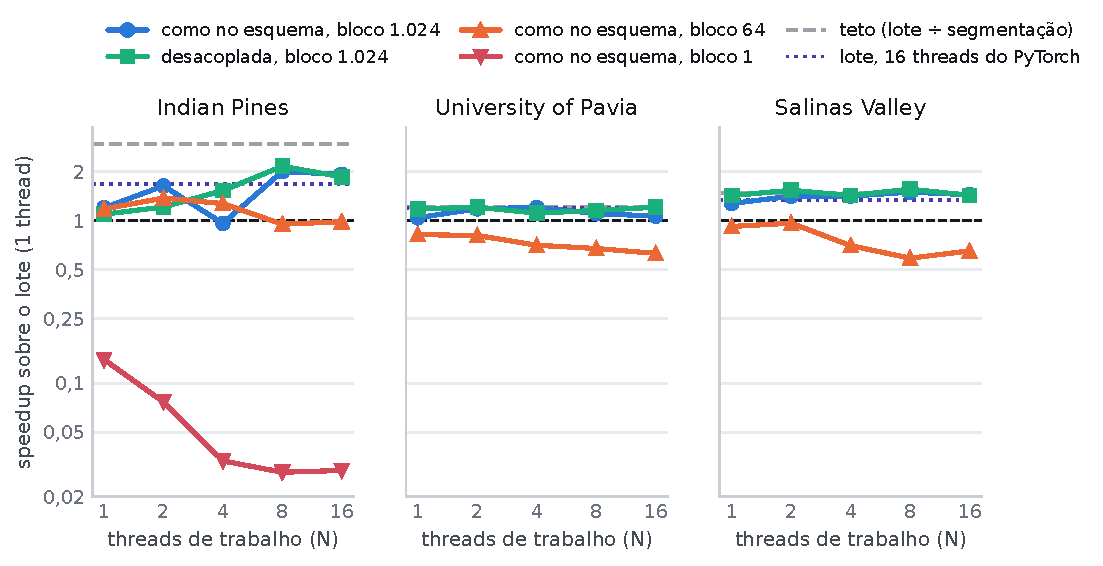
\includegraphics[width=\textwidth]{assets/resultados/fusao_speedup.pdf}
    \captionsetup{justification=raggedright}
    \caption*{Fonte: Elaborada pelo autor. Seção crítica como no esquema, a mesma do \autoref{qua:fusao}; as linhas de referência marcam o teto e o lote com 16 threads do PyTorch, e o eixo vertical está em escala logarítmica}
    \label{fig:fusaoSpeedup}
\end{figure}

Quatro leituras se destacam. A primeira é que, com a granularidade de uma posição por tarefa, o esquema fica de 7 a 35 vezes mais lento que o lote: em Indian Pines, a inferência que o lote faz em 0,33 s leva 2,35 s com uma thread de trabalho e de 9,9 s a 11,6 s com quatro ou mais. A maior parte desse custo vem de chamar a rede inteira para um único pixel, pois a execução sequencial com blocos de uma posição, sem threads, já leva 1,03 s, 3,12 vezes o tempo do lote. Com threads, a disputa pelo GIL agrava a perda, e a própria segmentação em T0, que disputa o mesmo GIL, fica duas a quatro vezes mais lenta.

A segunda é que, com blocos maiores, o esquema atinge o teto em University of Pavia e Salinas Valley. Com blocos de 1.024 posições, o tempo de parede nessas cenas fica a poucos centésimos de segundo do tempo da segmentação: toda a inferência acontece enquanto T0 segmenta ou logo depois, nas threads de trabalho, e o \textit{speedup} chega a 1,21$\times$ e 1,50$\times$, contra tetos de 1,21$\times$ e 1,49$\times$. Como o teto foi calculado com o tempo médio da segmentação, que varia entre execuções, distâncias de poucos por cento a ele, para cima ou para baixo, estão dentro dessa variação. Em Indian Pines, onde a segmentação é curta, as $N$ threads também dividem a inferência entre si, e o esquema chega a 2,01$\times$, ainda distante do teto de 2,98$\times$; a série dessa cena não é monotônica, e com 4 threads, em que a segmentação levou em média 0,27 s, mais que o dobro das demais configurações, o \textit{speedup} cai para 0,96$\times$. Com blocos de 64 posições, as 669 tarefas de University of Pavia e as 846 de Salinas Valley já tornam o esquema mais lento que o lote.

A terceira diz respeito à sobreposição. A \autoref{fig:fusaoLinhaTempo} mostra a linha do tempo de uma execução em University of Pavia, na forma como no esquema e na variante desacoplada. Na forma como no esquema, cada thread de trabalho faz as convoluções do primeiro bloco e fica bloqueada à espera do mapa; enquanto T0 segmenta, só $N$ blocos avançam. Em University of Pavia e Salinas Valley, a fração das convoluções terminadas antes da publicação do mapa vai de 0,1\%, em Salinas Valley com blocos de 64 posições e uma thread de trabalho, a 38\%, em University of Pavia com blocos de 1.024 posições e 16 threads; em Indian Pines, com 16 threads e blocos de 1.024 posições, os $N$ primeiros blocos já cobrem a cena inteira. Na variante desacoplada, em University of Pavia e Salinas Valley, todas as convoluções terminam durante a segmentação; em Indian Pines, onde a segmentação é curta, isso só ocorre com mais de uma thread de trabalho e blocos de 64 ou 1.024 posições (com uma thread, terminam em média 91\% e 94\% delas, e com blocos de uma posição, de 3\% a 13\%).

\begin{figure}[H]
    \centering
    \captionsetup{justification=centering}
    \caption{Linha do tempo de uma execução da fusão concorrente em University of Pavia, como no esquema e na variante desacoplada (4 threads de trabalho, blocos de 64 posições)}
    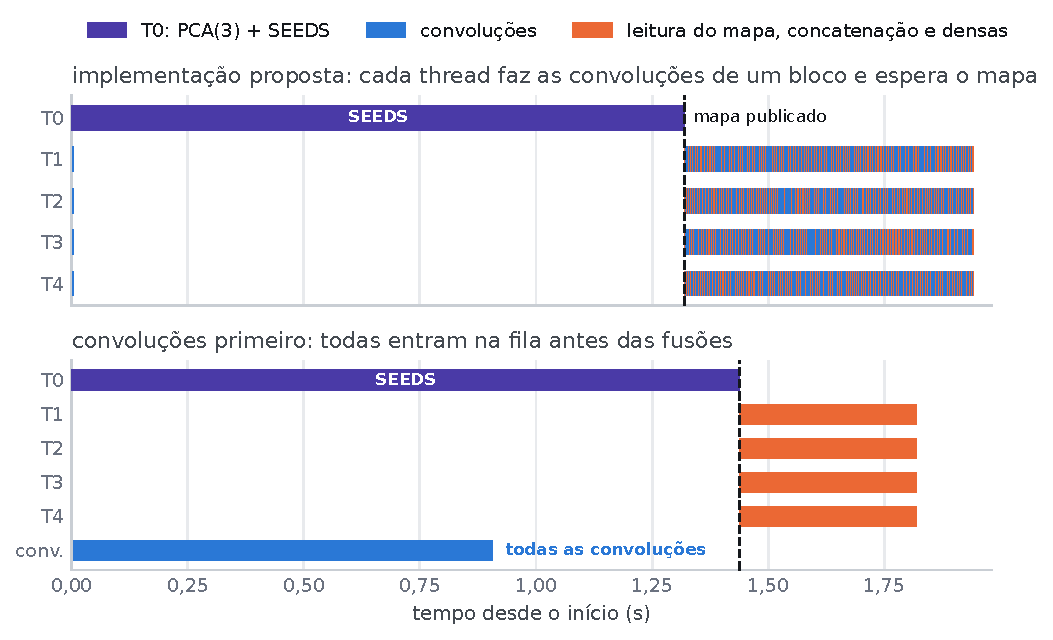
\includegraphics[width=\textwidth]{assets/resultados/fusao_linha_do_tempo.pdf}
    \captionsetup{justification=raggedright}
    \caption*{Fonte: Elaborada pelo autor. Execuções isoladas; a segmentação levou 1,10 s na forma como no esquema e 0,90 s na variante desacoplada}
    \label{fig:fusaoLinhaTempo}
\end{figure}

Na execução da figura, com blocos de 64 posições, o restante leva 0,62 s na forma como no esquema e 0,32 s na variante desacoplada depois da publicação do mapa; a diferença no tempo total (1,72 s contra 1,22 s) também reflete a segmentação, que levou 1,10 s e 0,90 s nessas duas execuções, e nas médias de 5 repetições a diferença é de 1,48 s contra 1,25 s. Com blocos de 1.024 posições, as duas formas ficam próximas em University of Pavia e Salinas Valley (\autoref{qua:fusao}), porque depois da publicação as $N$ threads concluem rapidamente o restante. Em Indian Pines, onde a segmentação é curta, o ganho vem sobretudo de dividir a inferência entre threads; em University of Pavia e Salinas Valley, a variante desacoplada com uma única thread de trabalho, que só antecipa as convoluções, já fica perto do teto (1,18$\times$ e 1,43$\times$). A extensão da seção crítica também não fez diferença mensurável: as duas versões ficaram dentro da variação entre repetições, e travar a concatenação não chegou a serializar as threads de forma visível.

A quarta leitura põe o resultado em perspectiva. Contra o lote executado com as 16 threads internas do PyTorch, que é o paralelismo dentro de cada operação já oferecido pela biblioteca, a melhor configuração com blocos de 1.024 posições rende de 1,01$\times$, em University of Pavia, a 1,29$\times$, em Indian Pines, uma economia de 0,01 s a 0,10 s por cena. Além disso, a inferência é uma parte pequena de uma execução completa, dominada pelo treino. O esquema é, portanto, uma forma correta e verificada de executar a proposta do projeto. Seu ganho aparece no cenário em que um modelo já treinado classifica uma cena nova, no qual segmentação e inferência são todo o trabalho, e fica entre 1,01$\times$ e 1,29$\times$ contra o lote com 16 threads; é limitado pelo tempo da segmentação e não tem efeito sobre o treino.

\section{Automação de Hiperparâmetros}
\label{sec:resHPO}

\subsection{Estratégias de Busca}

O \autoref{qua:estrategias} e a \autoref{fig:estrategias} comparam as três estratégias com o mesmo espaço, o mesmo número de \textit{trials} (20), a mesma cobertura inicial e três orçamentos de épocas por \textit{trial}, em Indian Pines, com 3 sementes por célula (540 \textit{trials} ao todo). A métrica de seleção é a melhor acurácia de validação; a OA de teste do vencedor é apenas relatada.

\begin{quadro}[H]
    \centering
    \caption{Estratégias de busca por orçamento de épocas (Indian Pines, 3 sementes)}
    \begin{tabular}{|p{0.16\textwidth}|p{0.14\textwidth}|c|c|}
        \hline
        \rowcolor[HTML]{C0C0C0}
        \textbf{Orçamento} & \textbf{Estratégia} & \textbf{Melhor validação} & \textbf{OA de teste do vencedor} \\
        \hline
        10 épocas & Aleatória & 0,7174 $\pm$ 0,0027 & 0,7065 \\
                  & TPE & 0,7226 $\pm$ 0,0162 & 0,7130 \\
                  & Genética & 0,7334 $\pm$ 0,0199 & 0,7174 \\
        \hline
        40 épocas & Aleatória & 0,7802 $\pm$ 0,0156 & 0,7729 \\
                  & TPE & 0,7924 $\pm$ 0,0193 & 0,7997 \\
                  & Genética & 0,8058 $\pm$ 0,0114 & 0,7989 \\
        \hline
        200 épocas & Aleatória & 0,8067 $\pm$ 0,0149 & 0,7859 \\
                   & TPE & 0,8266 $\pm$ 0,0175 & 0,8127 \\
                   & Genética & 0,8288 $\pm$ 0,0346 & 0,8080 \\
        \hline
    \end{tabular}
    \captionsetup{justification=raggedright}
    \caption*{Fonte: Elaborado pelo autor}
    \label{qua:estrategias}
\end{quadro}

\begin{figure}[H]
    \centering
    \captionsetup{justification=centering}
    \caption{Melhor acurácia de validação por estratégia e orçamento de épocas}
    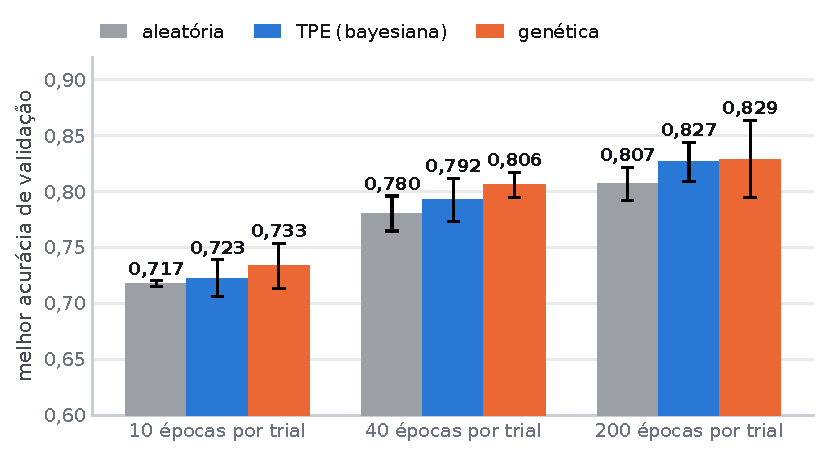
\includegraphics[width=0.85\textwidth]{assets/resultados/estrategias_hpo.pdf}
    \captionsetup{justification=raggedright}
    \caption*{Fonte: Elaborada pelo autor}
    \label{fig:estrategias}
\end{figure}

Nenhuma estratégia se separa das outras além do ruído entre sementes. As adaptativas (TPE e genética) ficam à frente da busca aleatória em todos os orçamentos, mas a diferença máxima, de 2,56 pontos com 40 épocas, é da mesma ordem do desvio médio entre sementes, de 1,3 a 2,2 pontos conforme o orçamento. Nas condições medidas (Indian Pines, 10\% do treino, 20 \textit{trials} e 3 sementes), o que mais mudou o resultado foi o orçamento: passar de 10 para 200 épocas por \textit{trial} acrescenta de 9 a 10 pontos à melhor validação, para qualquer estratégia, e a busca aleatória com 200 épocas empata com as estratégias adaptativas com 40 e supera as três com 10. Com um espaço em que poucos hiperparâmetros dominam, o sorteio já encontra a região de bons resultados, como previsto por \citeonline{Bergstra2012Random}, e o que limita a busca é quanto cada candidato pode treinar.

\subsection{Peso de Cada Hiperparâmetro}

A \autoref{fig:eixos} mostra a acurácia de validação média dos 540 \textit{trials} por valor de cada hiperparâmetro. O \textit{dropout} é o hiperparâmetro mais influente, com 18,10 pontos entre o melhor e o pior valor, seguido da taxa de aprendizado (15,26), do número de componentes do PCA (8,35), do \textit{weight decay} (4,55) e do tamanho do lote (1,81). O segmentador, que também faz parte do espaço de busca e não aparece na figura, separa 14,89 pontos nessa mesma medida, com o SEEDS à frente. A receita herdada usa o pior valor do hiperparâmetro mais influente: o \textit{dropout} de 0,5 fica 18,10 pontos abaixo do de 0,20. Nas condições medidas, com 10\% do treino em uma única cena, regularizar demais foi o erro mais caro. Essas médias, porém, misturam \textit{trials} de três orçamentos de épocas, escolhidos por estratégias diferentes, e não isolam o efeito de cada hiperparâmetro.

\begin{figure}[H]
    \centering
    \captionsetup{justification=centering}
    \caption{Acurácia de validação média por valor de cada hiperparâmetro do espaço de busca, com o valor herdado destacado}
    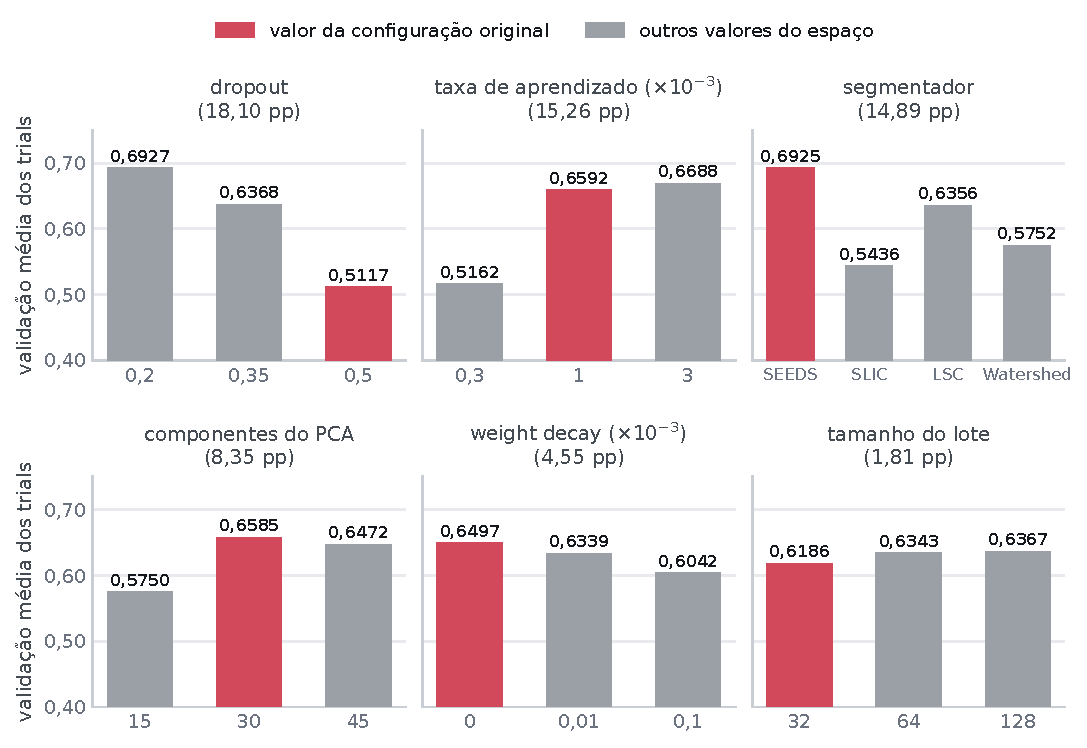
\includegraphics[width=\textwidth]{assets/resultados/eixos_hpo.pdf}
    \captionsetup{justification=raggedright}
    \caption*{Fonte: Elaborada pelo autor. Taxa de aprendizado e \textit{weight decay} em unidades de $10^{-3}$; entre parênteses, a diferença entre o melhor e o pior valor de cada hiperparâmetro, em pontos percentuais}
    \label{fig:eixos}
\end{figure}

\subsection{Ganho sobre a Receita Herdada}

O \autoref{qua:impactoHPO} e a \autoref{fig:impactoHPO} respondem à pergunta central deste eixo: quanto se ganha ao substituir a receita herdada pela receita encontrada pela busca. Para cada segmentador, as duas receitas foram treinadas com as mesmas 5 sementes, em Indian Pines, com 10\% do treino. A receita herdada é a do notebook original --- taxa de aprendizado 0,001, \textit{dropout} 0,5, \textit{weight decay} 0, lote 32 e 30 componentes ---, e a otimizada é a vencedora da busca TPE do mesmo segmentador (\autoref{ap:receitas}); as duas são treinadas com a regra de parada da \autoref{subsec:desTreino}. Um ganho é considerado afirmável quando excede duas vezes o desvio combinado das duas receitas entre sementes.

\begin{quadro}[H]
    \centering
    \caption{Receita herdada contra receita otimizada (Indian Pines, 5 sementes, 10\% do treino)}
    \resizebox{\textwidth}{!}{%
    \begin{tabular}{|l|c|c|c|c|l|}
        \hline
        \rowcolor[HTML]{C0C0C0}
        \textbf{Segmentador} & \textbf{OA herdada} & \textbf{OA otimizada} & \textbf{Ganho (pp)} & \textbf{Desvio comb.} & \textbf{Leitura} \\
        \hline
        SEEDS (herdado) & 0,7441 $\pm$ 0,0169 & 0,8174 $\pm$ 0,0112 & +7,33 & 2,03 & afirmável \\
        \hline
        SLIC & 0,6060 $\pm$ 0,1603 & 0,6411 $\pm$ 0,1856 & +3,51 & 24,53 & ruído \\
        \hline
        LSC & 0,6814 $\pm$ 0,0381 & 0,7566 $\pm$ 0,0219 & +7,52 & 4,39 & ruído \\
        \hline
        Watershed & 0,5847 $\pm$ 0,1586 & 0,5646 $\pm$ 0,2255 & $-$2,00 & 27,57 & ruído \\
        \hline
    \end{tabular}%
    }
    \captionsetup{justification=raggedright}
    \caption*{Fonte: Elaborado pelo autor}
    \label{qua:impactoHPO}
\end{quadro}

\begin{figure}[H]
    \centering
    \captionsetup{justification=centering}
    \caption{OA de teste com a receita herdada (lote 32) e com a receita otimizada, por segmentador (Indian Pines, 5 sementes, 10\% do treino)}
    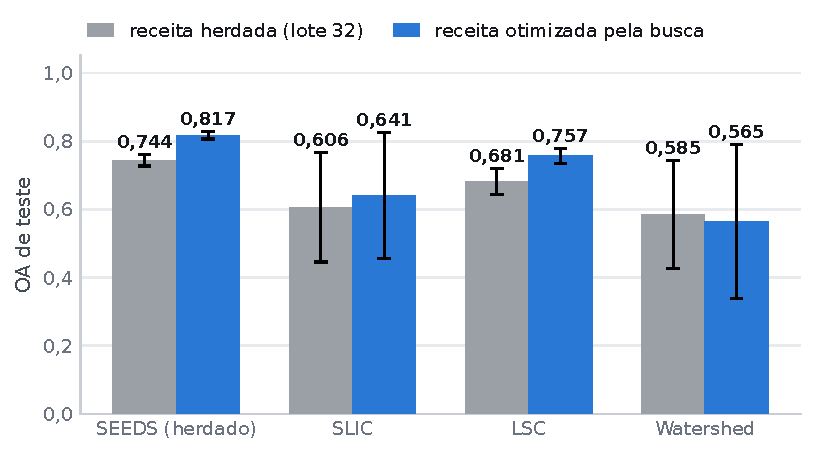
\includegraphics[width=0.85\textwidth]{assets/resultados/impacto_hpo.pdf}
    \captionsetup{justification=raggedright}
    \caption*{Fonte: Elaborada pelo autor. As barras de erro indicam o desvio padrão entre sementes}
    \label{fig:impactoHPO}
\end{figure}

Na configuração do trabalho de referência, com o SEEDS, a busca acrescenta 7,33 pontos de OA, 10,81 de AA e 8,52 de Kappa, e esse é o único ganho deste eixo que se separa do ruído entre sementes; na AA, por margem mínima, já que o limiar, de duas vezes o desvio combinado, é de 10,78 pontos. A receita vencedora reduz o \textit{dropout} de 0,5 para 0,35, dobra o tamanho do lote e usa 15 componentes do PCA em vez de 30, mantendo a taxa de aprendizado herdada. A redução do \textit{dropout} é coerente com o peso dos hiperparâmetros medido acima, em que o valor herdado é o pior do hiperparâmetro mais influente, enquanto a escolha de 15 componentes não é, pois esse é o pior valor médio do número de componentes do PCA; como as três mudanças vieram juntas, o efeito de cada uma não foi isolado. Para os demais segmentadores, o desvio entre sementes é grande demais para afirmar o sinal do ganho: SLIC e Watershed colapsam em algumas sementes com qualquer das duas receitas, e o ganho do LSC, de 7,52 pontos, fica abaixo do limiar de 8,78. Esse ganho foi medido com 10\% do treino, que é o regime em que a busca foi feita. Com o treino completo, apenas a configuração herdada foi medida, e seus valores absolutos são os do \autoref{qua:linhaBase}; o efeito da receita otimizada nesse regime não foi medido.

\section{Segmentadores}
\label{sec:resSegmentadores}

\subsection{O que Cada Algoritmo Produz}

O \autoref{qua:estruturaSeg} resume a estrutura das segmentações com os parâmetros padrão. O SEEDS produz poucas regiões grandes (81 em Indian Pines e 45 em University of Pavia), enquanto SLIC e LSC produzem quatro vezes mais regiões em Indian Pines e cerca de trinta vezes mais em University of Pavia. A pureza, isto é, a fração da classe dominante dentro de cada região, é maior no LSC e no SLIC. Todos os algoritmos são rápidos em relação ao treino; o SEEDS é o mais lento nas duas cenas, e o Watershed, o mais rápido.

\begin{quadro}[H]
    \centering
    \caption{Estrutura das segmentações com os parâmetros padrão}
    \begin{tabular}{|l|l|c|c|c|c|}
        \hline
        \rowcolor[HTML]{C0C0C0}
        \textbf{Cena} & \textbf{Algoritmo} & \textbf{Regiões} & \textbf{Área média (px)} & \textbf{Pureza} & \textbf{Tempo (s)} \\
        \hline
        Indian Pines & SEEDS & 81 & 259,6 & 0,8831 & 0,149 \\
                     & SLIC & 324 & 64,9 & 0,9581 & 0,051 \\
                     & LSC* & 324 & 64,9 & 0,9699 & 0,031 \\
                     & Watershed & 273 & 77,0 & 0,8543 & 0,004 \\
        \hline
        University of Pavia & SEEDS & 45 & 4.608,9 & 0,9212 & 1,854 \\
                    & SLIC & 1.428 & 145,2 & 0,9857 & 0,263 \\
                    & LSC* & 1.428 & 145,2 & 0,9955 & 0,203 \\
                    & Watershed & 421 & 492,6 & 0,9313 & 0,030 \\
        \hline
    \end{tabular}
    \captionsetup{justification=raggedright}
    \caption*{Fonte: Elaborado pelo autor. * LSC medido antes da correção do seu não determinismo. Tempos de uma medição avulsa dos segmentadores isolados, em sessão distinta; não são comparáveis aos do \autoref{qua:ramos} nem aos da \autoref{subsec:resFusao}, em que o SEEDS leva cerca de 0,11 s em Indian Pines e 0,87 s em University of Pavia}
    \label{qua:estruturaSeg}
\end{quadro}

\subsection{A Comparação com a CNN Fixa}

A primeira comparação, prevista no plano de verificação, manteve os hiperparâmetros da CNN fixos para os quatro segmentadores. Em University of Pavia, o SEEDS obteve Kappa de 0,9360, enquanto o SLIC obteve 0,0346, praticamente o de um classificador aleatório, e o LSC, 0,1970 com desvio de 0,35 entre sementes (medido antes da correção do seu não determinismo). A explicação está na escala da segunda entrada: com 1.428 regiões, o identificador concatenado vai até 1.428, contra componentes espectrais de variância unitária, e a receita que serve ao SEEDS, com 45 regiões, não serve a esses algoritmos. Algumas sementes treinam e outras colapsam, o que explica o desvio. A conclusão que esse desenho sugeriria, de que o SLIC não serve para University of Pavia, é desmentida pela otimização conjunta a seguir, e o desenho foi mantido apenas como contraexemplo.

\subsection{Sob Otimização Conjunta}

O \autoref{qua:segmentadores} e a \autoref{fig:segmentadores} mostram a OA de cada segmentador quando a CNN é otimizada para ele, com o mesmo orçamento de busca, nas três cenas. As receitas vencedoras estão no \autoref{ap:receitas}.

\begin{quadro}[H]
    \centering
    \caption{OA de teste de cada segmentador sob otimização conjunta (5 sementes, 10\% do treino)}
    \resizebox{\textwidth}{!}{%
    \begin{tabular}{|l|c|c|c|c|}
        \hline
        \rowcolor[HTML]{C0C0C0}
        \textbf{Cena} & \textbf{SEEDS (herdado)} & \textbf{SLIC} & \textbf{LSC*} & \textbf{Watershed} \\
        \hline
        Indian Pines & 0,8174 $\pm$ 0,0112 & 0,6411 $\pm$ 0,1856 & 0,7446 $\pm$ 0,0284 & 0,5646 $\pm$ 0,2255 \\
        \hline
        University of Pavia & 0,9515 $\pm$ 0,0042 & 0,9534 $\pm$ 0,0039 & 0,9373 $\pm$ 0,0053 & 0,9555 $\pm$ 0,0020 \\
        \hline
        Salinas Valley & 0,9632 $\pm$ 0,0076 & 0,9501 $\pm$ 0,0045 & 0,9470 $\pm$ 0,0019 & 0,9497 $\pm$ 0,0046 \\
        \hline
    \end{tabular}%
    }
    \captionsetup{justification=raggedright}
    \caption*{Fonte: Elaborado pelo autor. * LSC medido antes da correção do seu não determinismo; após a correção, em Indian Pines, a mesma receita obteve 0,7566 $\pm$ 0,0219}
    \label{qua:segmentadores}
\end{quadro}

\begin{figure}[H]
    \centering
    \captionsetup{justification=centering}
    \caption{OA de teste de cada segmentador sob otimização conjunta, por cena}
    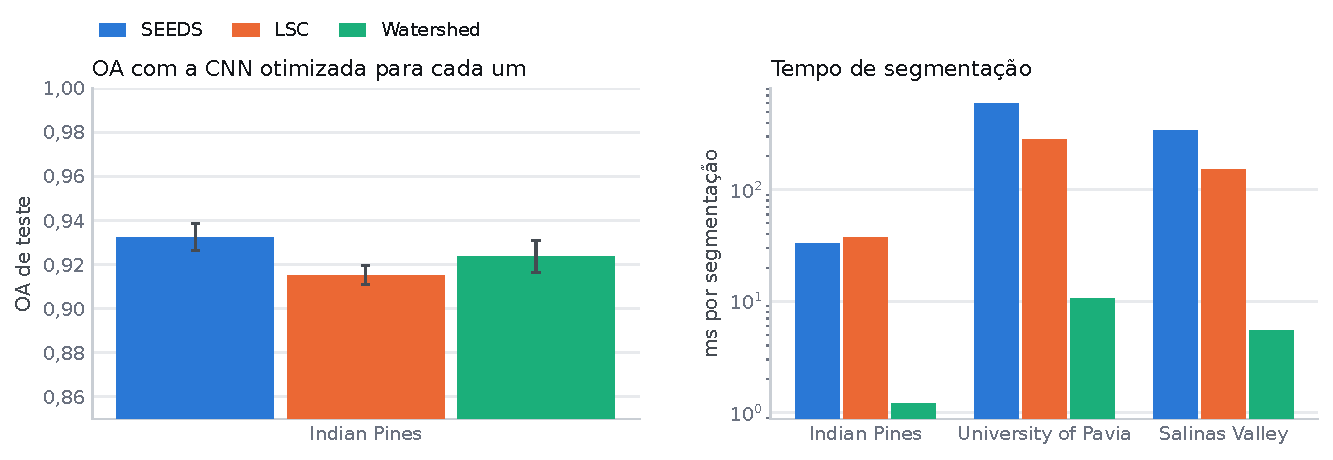
\includegraphics[width=\textwidth]{assets/resultados/segmentadores.pdf}
    \captionsetup{justification=raggedright}
    \caption*{Fonte: Elaborada pelo autor. WS: Watershed. * LSC medido antes da correção do seu não determinismo. A linha tracejada marca a OA do SEEDS, e as barras de erro, o desvio padrão entre sementes. Nos painéis de University of Pavia e Salinas Valley, o eixo vertical começa em 0,90}
    \label{fig:segmentadores}
\end{figure}

Desses resultados decorrem três conclusões. A primeira é que o segmentador é uma das escolhas de maior impacto do fluxo, embora com resultados instáveis. Em Indian Pines, 25,3 pontos de OA de teste separam o melhor do pior segmentador, cada um com a CNN otimizada para si; essa diferença, entre o SEEDS e o Watershed, vem sobretudo de duas sementes em que o Watershed colapsa e fica dentro do desvio, e a diferença afirmável nessa cena é a do SEEDS sobre o LSC, de 6,1 pontos com a receita refeita após a correção. Na análise por hiperparâmetro, que usa outra medida (a validação média por valor), o segmentador separa 14,89 pontos, atrás do \textit{dropout} (18,10) e da taxa de aprendizado (15,26).

A segunda é que nenhum segmentador supera o SEEDS herdado de forma afirmável. Em Indian Pines, todos ficam atrás mesmo otimizados para si, SLIC e Watershed com desvio muito alto; em University of Pavia, SLIC e Watershed têm média maior que a do SEEDS (+0,19 e +0,41 ponto), dentro do desvio; em Salinas Valley, SLIC e Watershed ficam 1,3 ponto atrás, também dentro do desvio, e só o LSC (1,6 ponto atrás) passa do critério, por margem mínima. Em University of Pavia e Salinas Valley, a meta de validação de 0,95 interrompe cedo parte dos treinos (em média, 2,8 épocas no SEEDS em Salinas Valley; \autoref{ap:receitas}), e diferenças dessa ordem devem ser lidas com essa ressalva.

A terceira é que cada segmentador escolhe hiperparâmetros diferentes: em Indian Pines, o SLIC foi o único a escolher uma taxa de aprendizado três vezes menor e lotes de 128, o que é coerente com a necessidade de acomodar um identificador de escala maior, que, com as regiões de 5 px da receita vencedora, vai até cerca de 840. O segmentador reconfigura o treino, e por isso não pode ser comparado com a CNN fixa.

\subsection{O que Explica o Desempenho}

A pureza das regiões não acompanha o resultado: em Indian Pines, o LSC tem a maior pureza (0,97, medida antes da correção do seu não determinismo) e fica 6,1 pontos atrás do SEEDS com a receita refeita após a correção (7,3 pontos na medição anterior), enquanto a pureza do SEEDS, de 0,88, só supera a do Watershed. O resultado é compatível com o número de amostras de treino por região: com os parâmetros padrão e 10\% do treino, são 10,8 no SEEDS, contra 2,7 no SLIC e no LSC e 3,2 no Watershed, e as receitas vencedoras do SLIC e do LSC, com regiões de 5 px, ficam perto de uma amostra por região (\autoref{qua:receitasVencedoras}). Com o treino fixo, porém, esse indicador é apenas o inverso do número de regiões, que também fixa a magnitude do identificador; ele não ordena os outros três algoritmos (o Watershed, com 3,2 amostras por região, tem a menor OA), e quatro algoritmos em uma única cena não permitem separar os dois efeitos nem afirmar uma causa.

O \autoref{qua:ablacao} ajuda a entender como o identificador é aproveitado. Cada linha altera uma propriedade do identificador do SEEDS, em Indian Pines, com 3 sementes. Substituí-lo por um número aleatório por pixel, que preserva apenas a escala, é a pior alteração, o que indica que a rede usa a informação de agrupamento. Normalizá-lo para o intervalo $[0, 1]$, que preserva tudo menos a magnitude, custa 7,58 pontos, o que indica que a rede se apoia na escala exagerada do identificador. Por fim, uma tabela de vetores aprendidos por região, que elimina tanto a ordem artificial entre identificadores quanto a dependência da escala, elevou a OA de 0,8981 para 0,9471 em Indian Pines e, na mesma comparação de modos de fusão, também com 3 sementes e fora do quadro, de 0,9785 para 0,9868 em University of Pavia. Sem o desvio registrado, essas diferenças não podem ser submetidas ao critério de afirmabilidade usado no restante do capítulo; elas sugerem, como melhoria da fusão herdada, trocar a concatenação do identificador por um vetor aprendido por região.

\begin{quadro}[H]
    \centering
    \caption{Como o identificador do superpixel é aproveitado pela rede (Indian Pines, 3 sementes)}
    \begin{tabular}{|p{0.32\textwidth}|p{0.40\textwidth}|c|}
        \hline
        \rowcolor[HTML]{C0C0C0}
        \textbf{Identificador} & \textbf{O que preserva} & \textbf{OA} \\
        \hline
        Original (herdado) & tudo & 0,8981 \\
        \hline
        Permutado entre regiões & agrupamento e escala; perde a ordem & 0,8552 \\
        \hline
        Normalizado para $[0, 1]$ & tudo menos a magnitude & 0,8223 \\
        \hline
        Aleatório por pixel & só a escala; perde o agrupamento & 0,7898 \\
        \hline
        Vetor aprendido por região & agrupamento, sem ordem nem escala & 0,9471 \\
        \hline
    \end{tabular}
    \captionsetup{justification=raggedright}
    \caption*{Fonte: Elaborado pelo autor. Médias de 3 sementes, sem o desvio registrado; a linha do vetor aprendido vem da comparação de modos de fusão, com a mesma referência. A referência (0,8981) vem de uma rodada própria e difere das médias do \autoref{qua:fracaoTreino} (0,9016) e do \autoref{qua:linhaBase} (0,9051, semente 42); as diferenças entre linhas devem ser lidas dentro deste quadro}
    \label{qua:ablacao}
\end{quadro}

\section{Verificação dos Requisitos}
\label{sec:resVerificacao}

A verificação segue o plano do \autoref{cap:proj}. O \autoref{qua:verifRF} e o \autoref{qua:verifRNF} resumem, para cada requisito, a situação e a evidência que a sustenta.

\begin{quadro}[H]
    \centering
    \caption{Verificação dos requisitos funcionais}
    \begin{tabular}{|p{0.08\textwidth}|p{0.13\textwidth}|p{0.69\textwidth}|}
        \hline
        \rowcolor[HTML]{C0C0C0}
        \textbf{Req.} & \textbf{Situação} & \textbf{Evidência} \\
        \hline
        \textbf{RF01} & Atendido & CNN 1D implementada conforme o \autoref{qua:camadas}; OA de 0,9051 a 0,9938 na configuração herdada (\autoref{qua:linhaBase}) \\
        \hline
        \textbf{RF02} & Atendido & SEEDS, SLIC, LSC e Watershed, com o mesmo formato de saída (\autoref{subsec:desSegmentadores}) e comparados no \autoref{qua:segmentadores} \\
        \hline
        \textbf{RF03} & Atendido & Concatenação do identificador do superpixel após o achatamento, com entrada de 1.025 posições na cabeça densa em Indian Pines; substituir o identificador por ruído com a mesma escala reduz a OA em 10,83 pontos, na média de 3 sementes, sem desvio registrado (\autoref{qua:ablacao}); a vantagem sobre a rede puramente espectral é a reportada por \citeonline{Souza2023} \\
        \hline
        \textbf{RF04} & Atendido & Busca aleatória, TPE e algoritmo genético (\autoref{sec:desHPO}); ganho de 7,33 pontos de OA sobre a receita herdada, em Indian Pines e com 10\% do treino (\autoref{qua:impactoHPO}) \\
        \hline
        \textbf{RF05} & Atendido em parte & OA, AA e Kappa; tempo de cada etapa e da inferência; número de parâmetros; memória retida por \textit{trial} e por processo; \textit{speedup} e seu teto teórico. O pico de memória durante o treino e a inferência, previsto no plano, não foi medido \\
        \hline
        \textbf{RF06} & Atendido & Entre os ramos (até 1,22$\times$), na fusão concorrente (até 2,01$\times$ contra o lote com uma thread do PyTorch, no teto em University of Pavia e Salinas Valley, e de 1,01$\times$ a 1,29$\times$ contra o lote com 16 threads) e por partição da cena (até 4,47$\times$) \\
        \hline
    \end{tabular}
    \captionsetup{justification=raggedright}
    \caption*{Fonte: Elaborado pelo autor}
    \label{qua:verifRF}
\end{quadro}

\begin{quadro}[H]
    \centering
    \caption{Verificação dos requisitos não funcionais}
    \begin{tabular}{|p{0.08\textwidth}|p{0.13\textwidth}|p{0.69\textwidth}|}
        \hline
        \rowcolor[HTML]{C0C0C0}
        \textbf{Req.} & \textbf{Situação} & \textbf{Evidência} \\
        \hline
        \textbf{RNF01} & Atendido & A mesma arquitetura do notebook original de \citeonline{Souza2023}, com os mesmos 37.577 parâmetros em University of Pavia \\
        \hline
        \textbf{RNF02} & Atendido & Toda a implementação em Python \\
        \hline
        \textbf{RNF03} & Atendido em parte & Treino com aceleração por GPU, em uma GPU local, e não no Google Colab ou em ambiente HPC \\
        \hline
        \textbf{RNF04} & Atendido & Fusão por concatenação do identificador ao vetor de características espectrais \\
        \hline
        \textbf{RNF05} & Atendido em parte & Com o SEEDS, em Indian Pines e com 10\% do treino, +7,33 pontos de OA, +10,81 de AA e +8,52 de Kappa sobre a receita herdada; nos demais segmentadores, o ganho fica dentro do ruído entre sementes \\
        \hline
        \textbf{RNF06} & Atendido em parte & Execuções repetidas com a mesma configuração produzem resultados idênticos; entre sementes, com o SEEDS, o desvio da OA fica entre 0,42 e 1,69 ponto, abaixo de 2, mas o da AA chega a 4,43 pontos em Indian Pines, e SLIC e Watershed em Indian Pines chegam a 22,55 pontos de OA \\
        \hline
        \textbf{RNF07} & Atendido & Redução de tempo medida nas três estratégias de paralelismo, contra a execução sequencial ou em lote no mesmo dispositivo (\autoref{sec:resParalelismo}) \\
        \hline
    \end{tabular}
    \captionsetup{justification=raggedright}
    \caption*{Fonte: Elaborado pelo autor}
    \label{qua:verifRNF}
\end{quadro}

O plano também fixou metas de acurácia por conjunto de dados (\autoref{tab:validacaoDatasets}), comparadas no \autoref{qua:metas} com a configuração herdada reimplementada, com o treino completo. A meta é atingida em Salinas Valley e não é atingida, nesta execução de semente única, em University of Pavia, por 0,28 ponto de OA, 0,56 de AA e 0,02 de Kappa, nem em Indian Pines, onde a distância é maior. A meta de Indian Pines, de 0,95 de OA, está acima do próprio valor reportado no trabalho de referência (0,9142), e o ganho de 7,33 pontos obtido pela busca de hiperparâmetros foi medido com 10\% do treino; o efeito da receita otimizada com o treino completo, que poderia aproximar Indian Pines da meta, não foi medido.

\begin{quadro}[H]
    \centering
    \caption{Metas de acurácia do projeto e valores obtidos com a configuração herdada (OA; AA; Kappa)}
    \begin{tabular}{|p{0.22\textwidth}|p{0.22\textwidth}|p{0.28\textwidth}|p{0.16\textwidth}|}
        \hline
        \rowcolor[HTML]{C0C0C0}
        \textbf{Cena} & \textbf{Meta} & \textbf{Obtido} & \textbf{Situação} \\
        \hline
        Indian Pines & 0,95; 0,93; 0,94 & 0,9051; 0,8237; 0,8914 & Não atingida \\
        \hline
        University of Pavia & 0,98; 0,97; 0,97 & 0,9772; 0,9644; 0,9698 & Não atingida \\
        \hline
        Salinas Valley & 0,97; 0,96; 0,96 & 0,9938; 0,9956; 0,9931 & Atingida \\
        \hline
    \end{tabular}
    \captionsetup{justification=raggedright}
    \caption*{Fonte: Elaborado pelo autor}
    \label{qua:metas}
\end{quadro}

\section{Discussão dos Resultados}
\label{sec:resDiscussao}

Nos eixos de desempenho, os resultados convergem para uma mesma observação: o ganho de cada otimização é limitado pela fração do trabalho que ela alcança e depende da referência contra a qual é medido. Nos eixos de acurácia, o que decidiu quais diferenças podem ser afirmadas foi o ruído entre sementes.

No paralelismo, a partição em processos e a fusão concorrente produzem os mesmos resultados que a execução sequencial e o lote, respectivamente, enquanto o treino de partições em threads não os repete, porque as threads compartilham o gerador aleatório (\autoref{sec:resOrganizacao}). O ganho de cada estratégia, porém, é limitado pela fração do tempo que ela alcança. O paralelismo entre os ramos do pré-processamento só atingiu o teto do próprio desenho em Salinas Valley, e esse teto é baixo porque a segmentação domina o pré-processamento, que por sua vez é menos de 1\% de uma execução. A fusão concorrente proposta pelo orientador atingiu, com blocos de 1.024 posições, o teto dado pela segmentação em University of Pavia e Salinas Valley, mas atua sobre a inferência, que também é uma parte pequena do total. O ganho expressivo, de até 4,47$\times$, veio de paralelizar o treino entre partições da cena com processos, em Indian Pines, com 16 partições e pool aquecido. Em todos os níveis, threads de Python só aceleraram o que acontece fora do interpretador: a segmentação e as operações do PyTorch sobre blocos grandes, e não o laço de treino nem chamadas pixel a pixel.

A forma de medir decidiu mais de uma conclusão deste eixo. Com o pool de processos criado dentro da medição, a partição parecia não ganhar nada com 16 partições; com o pool aquecido, entregou 4,47$\times$. Na primeira rodada da fusão concorrente, as operações do PyTorch em cada thread de trabalho usavam as 32 threads padrão do OpenMP, porque a restrição a uma thread, feita na thread principal, não se propaga às demais (\autoref{subsec:fusaoConcorrente}); em University of Pavia, com blocos de 64 posições e uma thread de trabalho, o esquema levava 7,3 s nessa rodada, descartada, contra 1,28 s depois da correção (\autoref{qua:fusao}). Nos dois casos, a correção veio de conferir a medição antes de interpretá-la.

Na automação de hiperparâmetros, o ganho de 7,33 pontos de OA sobre a receita herdada, medido em Indian Pines com 10\% do treino, é o resultado mais direto do trabalho em acurácia. Ele vem de uma receita que reduz o \textit{dropout}, dobra o lote e usa 15 componentes do PCA; o efeito de cada mudança não foi isolado, mas a redução do \textit{dropout} é coerente com o peso dos hiperparâmetros, em que o valor herdado é o pior do hiperparâmetro mais influente. A escolha da estratégia de busca, por outro lado, não fez diferença afirmável. Nas condições medidas, com uma cena, 10\% do treino, 20 \textit{trials} e 3 sementes, aumentar o orçamento de épocas por \textit{trial} pesou mais que trocar a estratégia: a busca aleatória com 200 épocas empatou com as estratégias adaptativas com 40 e superou as três com 10.

Nos segmentadores, a comparação com a CNN fixa, prevista no plano, levaria à conclusão falsa de que o SLIC não serve para University of Pavia; com a CNN otimizada para ele, o SLIC empata com o SEEDS nessa cena, e cada segmentador escolhe hiperparâmetros próprios. Mesmo com a CNN otimizada para cada um, nenhum dos três superou o SEEDS herdado de forma afirmável, e o resultado acompanha o número de amostras de treino por região mais do que a pureza das regiões, sem que os dados permitam afirmar uma causa.

A organização do código, por fim, é o que torna os demais resultados atribuíveis. Dois dos três defeitos descritos na \autoref{sec:resOrganizacao}, o não determinismo do LSC e o gerador aleatório compartilhado entre threads, só foram encontrados porque cada execução é reprodutível e cada experimento confere a repetibilidade das próprias medições; o terceiro, o piso de componentes do PCA, apareceu quando a campanha foi interrompida por um erro. Em relação ao trabalho de referência, a configuração herdada reimplementada fica abaixo dos valores reportados por \citeonline{Souza2023} --- por menos de 1 ponto de OA em Indian Pines e Salinas Valley, 1,6 ponto em University of Pavia e 7,2 pontos de AA em Indian Pines ---, o que é coerente com uma política de parada única para as três cenas, em vez de ajustes por conjunto de dados, e com uma única execução de cada lado.
